\chapter{Methodology}

\section{Introduction}
The purpose of this chapter is to explain how the Retrieval-Augmented Generation (RAG) pipelines were designed, implemented, and evaluated for this thesis. This chapter ties together the theoretical background on LLMs, semantic search, reranking, hybrid retrieval and HPC deployment to a very practical note book based system as it was implemented in the repository.

This project employs an experimental engineering approach to software development. 

First a baseline RAG pipeline is created and thereafter retrieval level improvements are added to controlled variants. In order to test whether variations in timing or answer quality are due to the retrieval and ranking strategy under examination, all variants use the same data set, question scenarios, logging procedures, and evaluation programs.

\section{Research Framework and Design}

The approach uses six primary RAG architecture families and one RAG vector-database variant that has been specifically tailored. All six RAG architecture families appear in FIGURE ~\ref{fig:six-rag-pipeline-variants}. The implemented variants include a basic in-memory pipeline, a Milvus vector-database pipeline, a tuned vector-database pipeline, a reranking pipeline, a hybrid retrieval pipeline, and a hybrid retrieval with reranking pipeline. The main focus is to evaluate how these choices affect retrieval quality, answer quality, and execution time. The result logs reflect this as \texttt{basic}, \texttt{vectordb}, \texttt{vectordb\_\allowbreak tuned}, \texttt{reranker}, \texttt{hybrid}, and \texttt{hybrid\_\allowbreak rerank}.

The comparison is based on a "local first" workflow. The notebooks will be run on local systems to test all aspects of the code, services, prompts, documentation generation, results logging and evaluation scripts. All of these workflows will then be ready to be run in the future on an \ac{HPC}. While the ultimate goal of running this on an \ac{HPC} is not to modify the \ac{RAG} logic of the system, it is expected that some retrieval strategies (such as those using shared resources, schedulers etc.) may behave differently depending on the specific characteristics of the HPC execution environment (storage locations etc.), compared to their performance when executing within a local environment.

By focusing on retrieving and ranking, and keeping the generator model consistent across experiments wherever possible, we can isolate and compare the effects of changing various components of our retrieval strategy; including dense retrieval, persistent vector storage, tuned chunking, reranking, sparse-dense hybrid retrieval and hybrid retrieval with reranking.

\section{Dataset and Input Documents}

The experiments utilize the OrchestrAI enterprise synthetic dataset that was created for the purpose of this project (stored inside the project directory). The dataset includes 54 \texttt{.docx} files which were organized within departmental directories: (i) Customer Support , (ii) Engineering, (iii) Finance, (iv) HR, (v) IT, (vi) Logistics, (vii) Product, (viii) Sales, (ix) Security, (x) {Q\&A} Handbooks. The contents of these .docx files include company policy descriptions, customer service procedure documentation, on-boarding workflow information, procurement process documentation, product development/production information, cross-function operational scenario documentation. 

Each Notebook utilizes the Haystack \texttt{DOCXTo\allowbreak Document} converter to load the same document set recursively. While documents are loaded, they are enriched with additional metadata – primarily the original source filename and department. This additional metadata will be useful in manually evaluating retrieved documents when the retrieved documents are saved to the \texttt{results.csv} for later comparison purposes. 

Once all documents have been loaded into memory, they are divided into separate chunks prior to being indexed. The primary in-memory index pipeline utilizes word-based chunks of 120 words in length with an overlapping chunk of 20 words. The Milvus supported vector database, reranking, hybrid, and hybrid reranking pipelines utilized 80-word chunks with an overlapping chunk of 20 words. A single variation of the Tuned Vector Database Indexing Pipeline changed this parameter to allow for larger chunks (of 200 words) with greater overlap (an overlapping chunk of 40 words), thereby enabling the ability to test/chunk-size as a controlled variable.

\section{System Architecture}

The developed system has followed the common \ac {RAG} architecture as illustrated in Fig.~\ref{fig:methodology-rag-architecture}. In this case, a query by the user was used to retrieve relevant fragments of documents, these retrieved fragments were then integrated into a prompt which was provided to the language model as input. This prompted the language model to generate an answer based upon that context.

\begin{figure}[htbp]
    \centering
    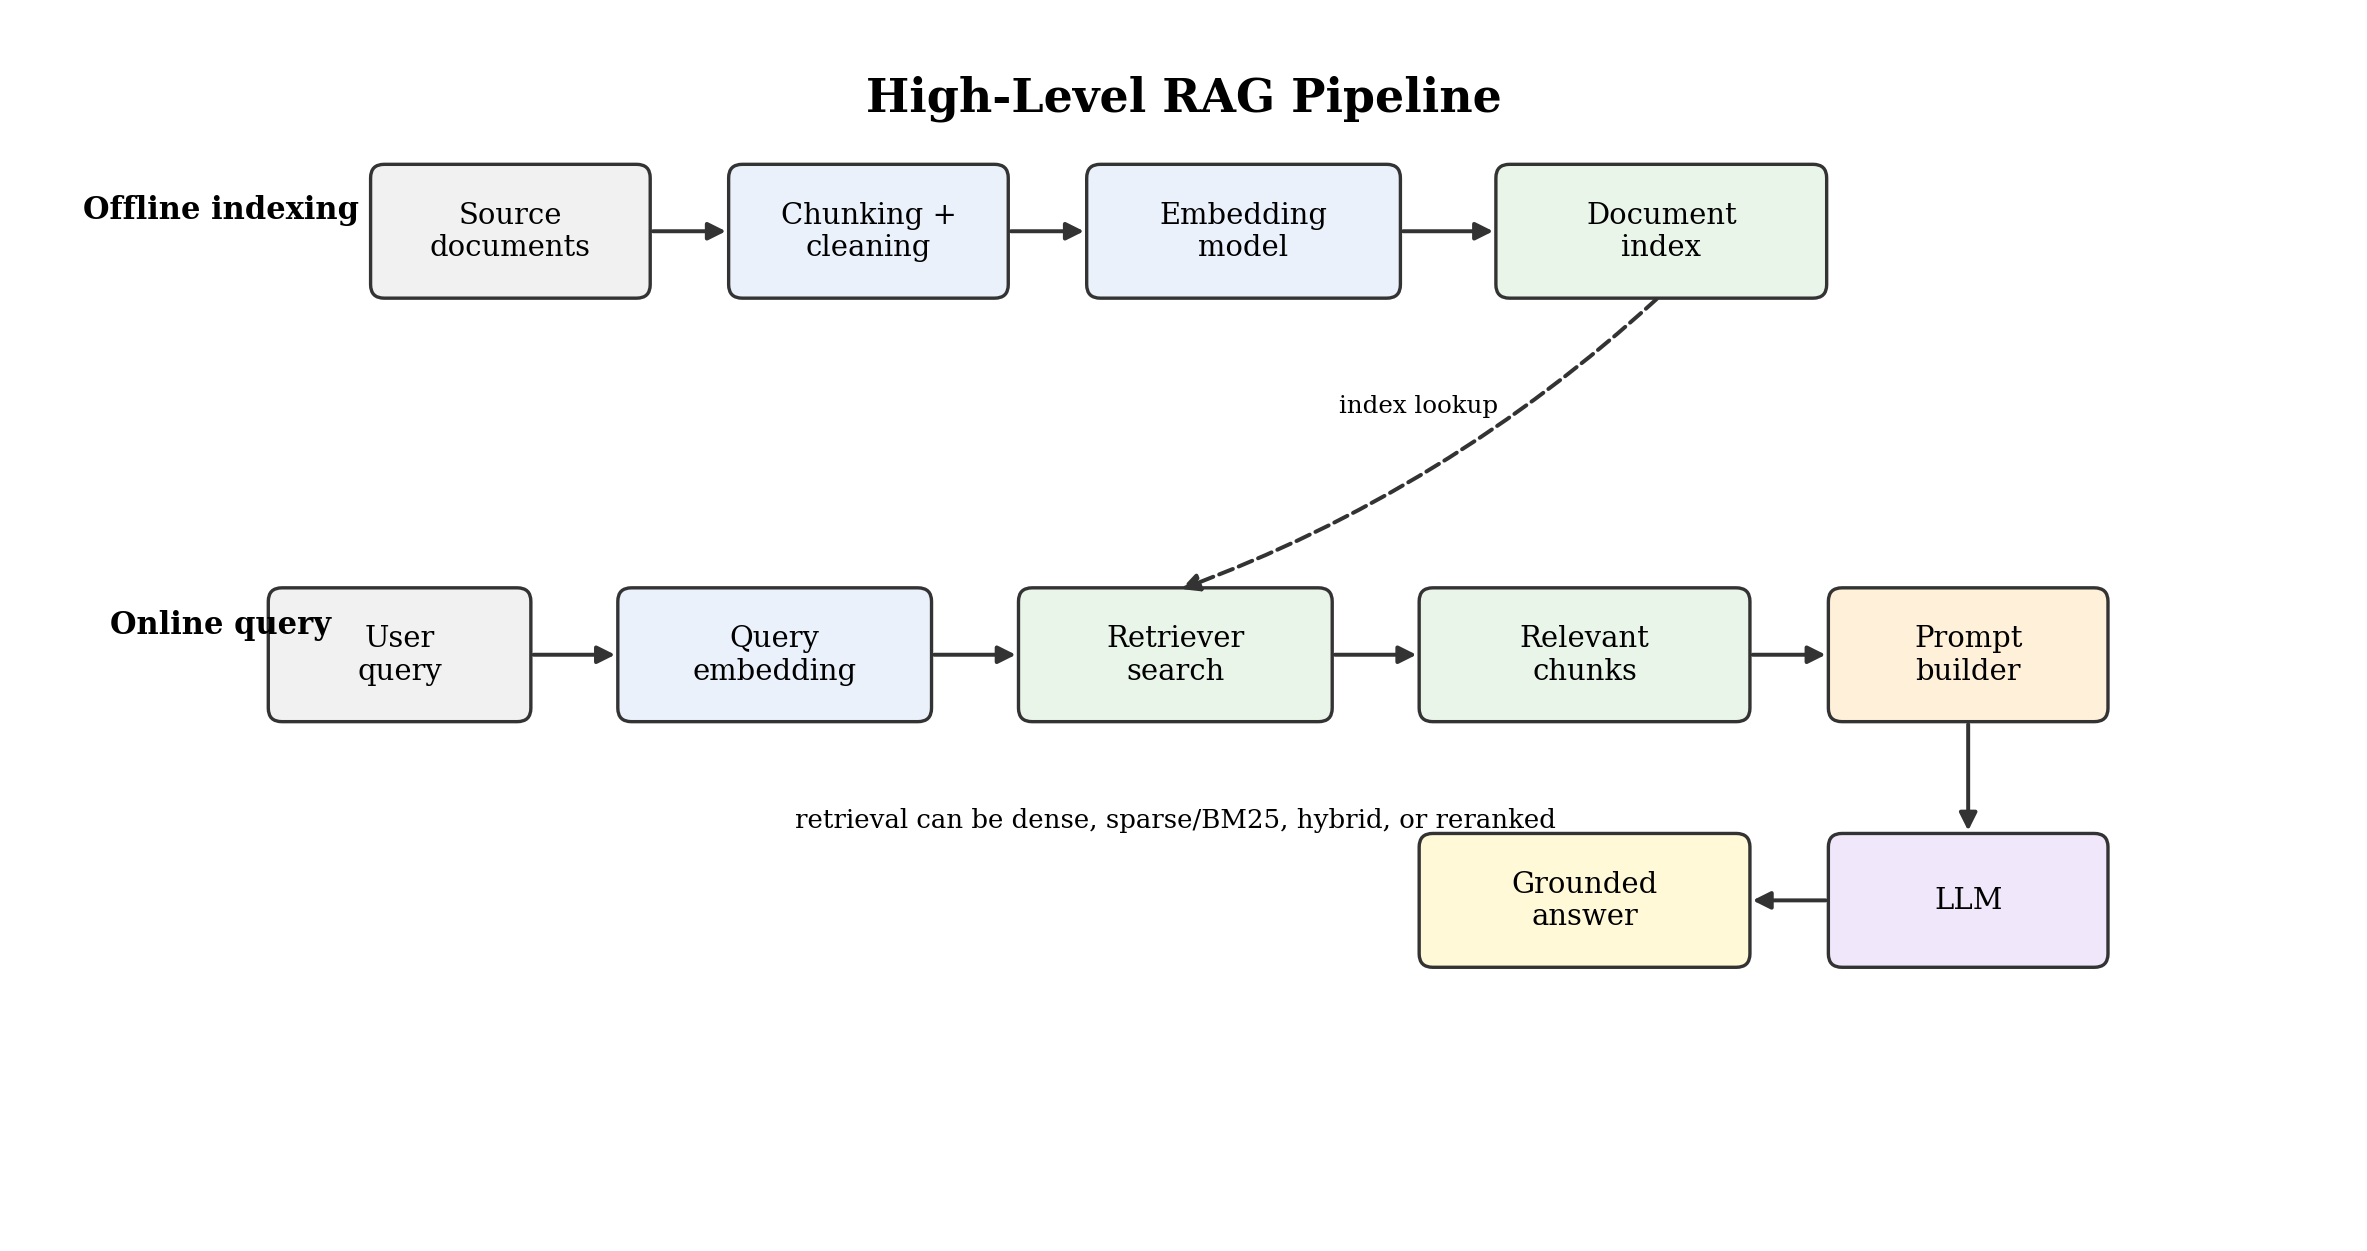
\includegraphics[width=0.9\textwidth]{images/fig03_high_level_rag_pipeline.png}
    \caption{High-level RAG workflow used by the implemented notebooks: user query, retrieval over indexed documents, context construction, and answer generation.}
    \label{fig:methodology-rag-architecture}
\end{figure}

Haystack components have been utilized in order to implement all aspects of the system, e.g. document conversion, splitting, embedding, retrieval, prompt construction, etc. Ollama has served as the host platform for both the answer generation model (\texttt{llama3.1}) and the embedding model (\texttt{mxbai-\_embed-\_large}). Since the embeddings used for dense retrieval are also created via use of the embedding model, a direct connection exists. The variant utilizing a local Milvus server connects directly to a local instance of the service. These services are managed via use of the stand-alone script \texttt{scripts/standalone\_embed.sh} within the project directory. Cross-encoding reranking utilizes a MiniLM cross-encoder trained upon \texttt{MS MARCO} ranking data.

The main architectural components are:

\begin{itemize}
    \item \textbf{Document Loader/Chunker:} Loads .docx files, saves source metadata from loaded documents and creates "chunks" that represent the document's content broken down by retrieval unit.
    \item \textbf{Embedding Model:} Converts each Document Chunk and User Question into a dense vector representation (e.g., embedding).
    \item \textbf{Document Store:} Stores each chunk in memory or uses a database like Milvus based on how the implementation was set up.
    \item \textbf{Retriever:} Uses Dense Vector Similarity or Hybrid Sparse-Dense Retrieval methods to find the best possible "candidate chunks".
    \item \textbf{Reranker:} Reorders the retrieved Candidate Chunks when using the Reranking variants before passing Context to Prompt.
    \item \textbf{Prompt Builder {\&} Generator:} Combines the Retrieved Context with the User's Question and sends the combined Question-Context pair to Llama3.1.
    \item \textbf{Results logger:} Writes the Implementation Name, Scenario Identifier, Retrieved Sources, Generated Answer and Timing Values to a shared CSV File.
\end{itemize}

By structuring the code in this way it allows for fair comparison since all Notebooks use the same high-level workflow but differ at the Retreival/Ranking strategy level. Also, this structure will allow for future HPC execution since all Notebooks and helper scripts may be executed in a managed environment with only environment specific setup changes.

\section{Implemented RAG Pipelines}

\begin{figure}[htbp]
    \centering
    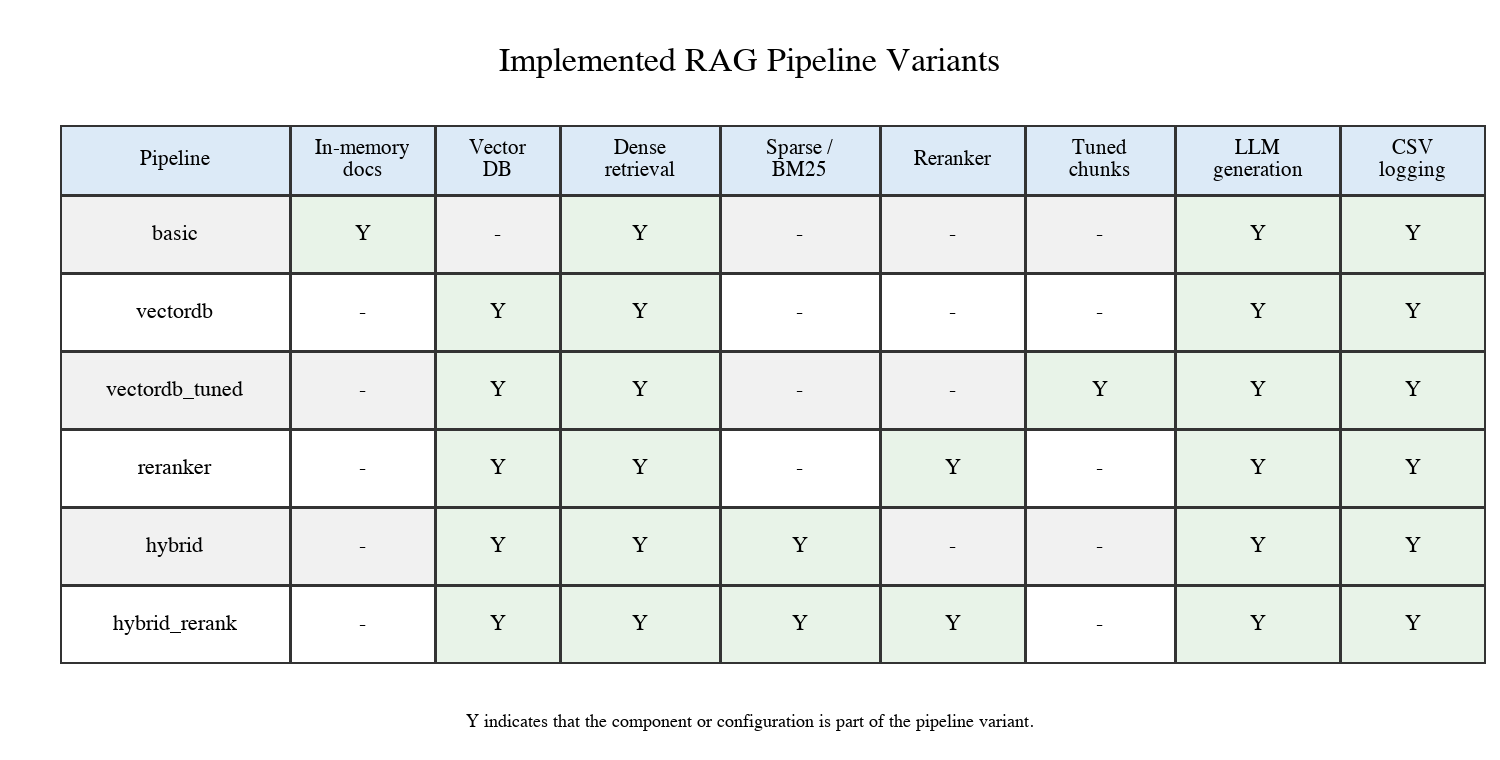
\includegraphics[width=\textwidth]{images/fig08_six_pipeline_variants.png}
    \caption{Comparison of the five RAG pipeline families implemented in the project: basic RAG, vector database RAG, reranking RAG, hybrid RAG, and hybrid RAG with reranking.}
    \label{fig:six-rag-pipeline-variants}
\end{figure}

\subsection{Baseline RAG version}
The baseline in-memory RAG version, \texttt{rag\_basic.ipynb}, utilizes an in-memory document store and an embedding based retriever. The goal of this pipeline was to provide the simplest completely working \ac{RAG} model and serve as a reference point for the other versions. It demonstrated how retrieval and generation work when there is no added overhead of a vector database, sparse retrieval, or reranking.

\subsection{Version Using a Vector Database RAG}

The vector-database version, \texttt{rag\_vectordb.ipynb}, places document embeddings into Milvus. For each query, the version queries the Milvus collection and returns the top 10 dense matches. This version tested the effects of utilizing persistent vector databases as opposed to in memory document stores.

\subsection{Tuned Version Using a Vector Database RAG}

The tuned vector-database version, \texttt{rag\_vectordb\_tuned.ipynb}, has the same Milvus backed dense retrieval structure as the standard vector-database pipeline. However, the primary differences were related to the chunking settings; specifically, the chunk size went up from 80 to 200 words while the chunk overlap increased from 20 to 40 words. This version evaluated if larger chunks would improve either retrieval behavior or answer quality.

\subsection{Reranking RAG}

The reranking version, \texttt{rag\_reranker.ipynb}, first retrieves 20 dense candidates via Milvus. Then those candidates are reordered using a cross-encoder reranker. Finally, the top 10 reranked candidates are sent to the generator. This version tested if adding another relevance order step to the initial set of retrieved content would improve its usefulness enough to justify the higher latency of performing two separate retrievals.

\subsection{Hybrid Retrieval RAG}

The hybrid version, \texttt{rag\_hybrid.ipynb}, used a hybrid retrieval mechanism made available by Milvus. A combination of dense semantic embeddings (i.e., semantic matching) and a sparse BM25 style representation produced inside Milvus (i.e., lexical matching). The goal of this version was to determine if semantic matching and lexical matching could be complementary. This is particularly interesting given that enterprise documents often contain exact term references (e.g., team name(s), severity level(s), product identifier(s), etc.).

\subsection{Hybrid Retrieval With Reranking RAG}

The hybrid-reranking version, \texttt{rag\_hybrid\_\&\_rerank.ipynb}, built upon the hybrid retrieval version. First, it retrieves 20 hybrid candidates. Next, it uses the cross-encoder reranker to select the top 10 documents for generation. While this version may enhance context ordering due to combining dense retrieval, sparse lexical matching, and reranking; it comes at a cost: the time needed to perform the retrieval will increase since both hybrid candidate retrieval and reranking occur prior to the actual generation of answers.

\subsection{Measured Variables}

We measure the following primary variables.

\begin{itemize} 
    \item Time to index in seconds
    \item Time to retrieve in seconds
    \item Time to generate in seconds
    \item Source files and departments that were retrieved
    \item Contexts that were retrieved
    \item Number of retrieved documents
    \item Top-k retriever and reranker values
    \item Generated answer text
    \item Correctness score and label given by manual assessment
    \item Deterministic measures of answer quality and retrieval quality. 
\end{itemize}

We have logged for future use all of the above (except for correctness assessments) as part of our current Results Logger: Implementation Name, Scenario ID, Question Asked, Answer Given, Sources Retrieved, Departments Retrieved, Contexts Retrieved, Number of Documents Retrieved, Top-k Values For Retriever and Reranker, Indexing Time, Retrieval Time, Generation Time. Manual correctness assessments and labels are included at some point after this has occurred, via the Ground-Truth Evaluation File. The evaluation script also produces deterministic metrics. The end-to-end response cost can be estimated using the total times for both retrieving and generating answers, however, we treat indexing time separately since it represents a cost associated with preparing the corpus before queries are run, whereas the other two represent costs associated with answering each query.

\section{Evaluation Framework}

\subsection{System Performance Metrics}
The overall system performance will be measured by timing that was collected from within the notebooks. The indexing time represents the total amount of time required by the system to prepare and save the chunks from documents. The retrieval time is used to represent how much time it takes to retrieve all the relevant chunks related to a specific scenario-based question. As mentioned previously, the reranking processes are considered to be part of the retrieval time in both cases. Finally, generation time indicates how long it takes for an LLM to generate a final response once the appropriate prompt is generated.

Timing values obtained while running locally will be saved to the experimental results CSV and subsequently to the final results directory.

% TODO: Complete this paragraph after the HPC experiment(s) have run.
% TODO: Add queue time, container start-up, service start-up, data-transfer time; 
% add node type, cpu/gpu allocation, memory allocation, scheduler parameters and storage path as well.

When comparing HPC systems with RAG systems, we anticipate collecting the same timing fields as before; however, we plan to collect additional timing fields which relate specifically to HPC (i.e., queue time, container start-up, service start-up, data-transfer time) in order to separate them from actual times associated with RAG pipeline execution time.

\subsection{Retrieval Quality Metrics}
Retrieval quality can be measured based on how well the model identifies true supporting documents compared to the manually selected supporting documents provided in the ground-truth CSV. In addition to calculating the proportion of manually selected supporting documents which were actually retrieved (recall), the proportion of all supporting documents retrieved that were also manually selected (precision) and an overall measure of balance between the two (F1). A "retrieval hit" exists when at least one manually selected supporting document is included in the list of retrieved sources.

\subsection{Answer Quality Metrics}
Manual evaluations assess the quality of the answer by providing a score to determine if the response was completely accurate, partially accurate, or completely inaccurate. Manual scoring is typically done by assigning a score of either 1.0 for fully correct, 0.5 for partially correct, and 0.0 for no correctness. 

In contrast to evaluating answer quality manually, the deterministic evaluation script calculates several additional metrics that can automatically measure aspects of answer quality. \ac{ROUGE-L} measures lexical overlap between the reference answer and the model's answer \cite{lin2004rouge}. \ac{BERTScore} measures the semantic similarity of the model's answer versus the reference answer \cite{zhang2020bertscore}. Similarly, a sentence transformer can measure the level of semantic similarity between individual sentences within each answer \cite{reimers2019sentencebert}. Additionally, there are metrics related to the retrieval quality of the model such as whether enough supporting documents were retrieved. Lastly, the deterministic evaluation script evaluates the length of each answer.

\subsection{Visual Analysis}
Visualizations are created through the use of a visualization notebook. After reading and processing all of the final results, it produces several types of figures that show answer quality, retrieval quality, per-scenario performance, timing breakdowns, and comparisons across multiple metrics. Each type of figure is then placed into its own subdirectory called "results figures." The figures created in this manner Figures~\ref{fig:methodology-rag-architecture} and~\ref{fig:six-rag-pipeline-variants} are used throughout the results chapter to demonstrate trade-offs made during implementation.

\subsection{Cross-Environment Comparison}

% TODO: Complete this subsection after the HPC experiments are executed.
% TODO: Add the HPC environment label, hardware metadata, scheduler settings,
% container setup, storage path, and service startup method.

\section{Reproducibility and Documentation}
Although the results logger module standardizes how results are collected by forcing each notebook to collect results in the same format, each notebook can still be run independently. Thus, each notebook represents a unique version of the RAG pipeline being tested. All other modules including the ground truth builder module that builds the evaluation template from generated results, and the deterministic evaluation module that compute all of the automated metrics are also independent.

Documentation is necessary for reproducibility. Therefore, there is a \texttt{README} document for setting up the software and running each notebook, along with documenting how to start Milvus and what Ollama models are required, how to execute each notebook, what command to run to perform evaluation, where output files are written etc. Local reproducibility is supported via this \texttt{README} document and serves as the foundation for future HPC installation instructions. For HPC reproduction purposes, documentation should include file transfers, environment configurations, scheduler commands, container/module selection options and/or output CSV file storage location(s).

\section{Summary}
This chapter described the methodology that was employed to test and evaluate the various RAG pipelines developed in this study. The chapter describes the experimental design for testing and evaluating these pipelines, defines how large a dataset was needed for training/testing, defines the corpora, outlines system architecture, lists out variations of each pipeline, describes variables that could affect results, describes how results would be evaluated, describes what types of visual outputs would be produced as part of analyzing results, and finally outlines how reproducible this study was.

In addition to describing methodology, this chapter provides the foundation upon which subsequent chapters build. The next chapter discusses how experiments were performed on these RAG pipelines.